\subsection{L2L2}

The following section discusses the events having no hit in Layer 1 of the 1.5~mm dataset. An additional requirement was made that the tracks must not project back to the active region of the Layer 1 silicon in order to avoid contamination by events with the Layer 1 inefficiency. 

\subsubsection{Cuts}

The cuts applied to the L2L2 dataset are shown in Table~\ref{l2l2_cuts_1p5}.

\begin{table}[H]
\caption{Cuts applied to the L2L2 datasets with the SVT at 1.5~mm.}
\label{l2l2_cuts_1p5}
\centering
\begin{tabular}{lllllll}
\toprule
%\multicolumn{2}{c}{Name} \\
%\cmidrule(r){1-2}
Cut type & Cut & Cut Value &  $\%$killed &  $\%$killed core & $\%$killed tails\\
\midrule
track & Fit quality & track $\chi^{2}<30$ & 29 & 11 & 39 \\
track & Max track momentum &  $P_{trk}<75\%E_{beam}$ & 10 & 8 & 12 \\
track & Isolation &   & 5 & 2 & 8 \\
vertex & beamspot constraint & bsc$\chi^{2}<10$  & 26 & 16 & 35 \\
vertex & beamspot - unconstrained & bsc$\chi^{2}$-unc$\chi^2<5$  & 10 & 8 & 14 \\
vertex & maximum $P_{sum}$ &  $<115\%E_{beam}$ & 1 & 1 & 1 \\
ecal & Ecal SVT matching & $\chi^2<10$  & 11 & 8 & 14 \\
ecal & track Ecal timing & $<4$ns  & 6 & 6 & 6 \\
ecal & 2 cluster time diff & $<2$ns  & 7 & 6 & 7 \\
physics & momentum asymmetry & $<0.4$  & 3 & 2 & 4 \\
physics & e+ track d0 & $<1.5$mm  & 9 & 7 & 12 \\
event & max shared hits amongst tracks & $<4$ shared hits  & 20 & 20 & 20 \\
\bottomrule
\end{tabular}
\end{table}

The cuts are the same as those applied to the data in the 0.5~mm L2L2 dataset. This dataset has significantly more statistics that needs to be studied and may complement the analysis on the 0.5~mm high z background data. 

\subsubsection{Vertex reconstruction efficiency, $\epsilon_{vtx}$}
The vertex reconstruction efficiency for the L2L2 dataset was fit at each simulated heavy photon mass using the Crystal Ball function in Equation~\eqref{eq:cbfunction}. The parameters are characterized as a function of mass in Equation~\eqref{eq:parsEpsVtxL2}.
\begin{eqnarray*}
\label{eq:parsEpsVtxL2}
z_{mean} & = & -45.49+5.25m-0.052m^2 \\
\sigma & = & 7+0.104m \\
N & = & -0.89+0.074m-0.000995m^2 \\
\end{eqnarray*}

The zMax for this dataset is 100~mm as the events can be reasonably reconstructed near Layer 1.

\subsubsection{Accidentals}

The out of time events as discussed previously were selected in order to understand the accidental rate. No accidental events were clearly identified, although some work is still necessary to understand the high z background when ublinding the dataset and optimizing the zCut. 

\subsubsection{Projected reach}
The L2L2 dataset is unique from other datasets in that it is most efficient at large z. Because of this geometric effect, we can identify and consider how the zCut changes at the low end of the efficiency as we move to large z by proposing cuts at the 2$\%$, 5$\%$, and 10$\%$ efficiency values. The corresponding zCut with this possibility is shown in Figure~\ref{fig:L2L2_zCut_1p5}.

\begin{figure}[H]
  \centering
     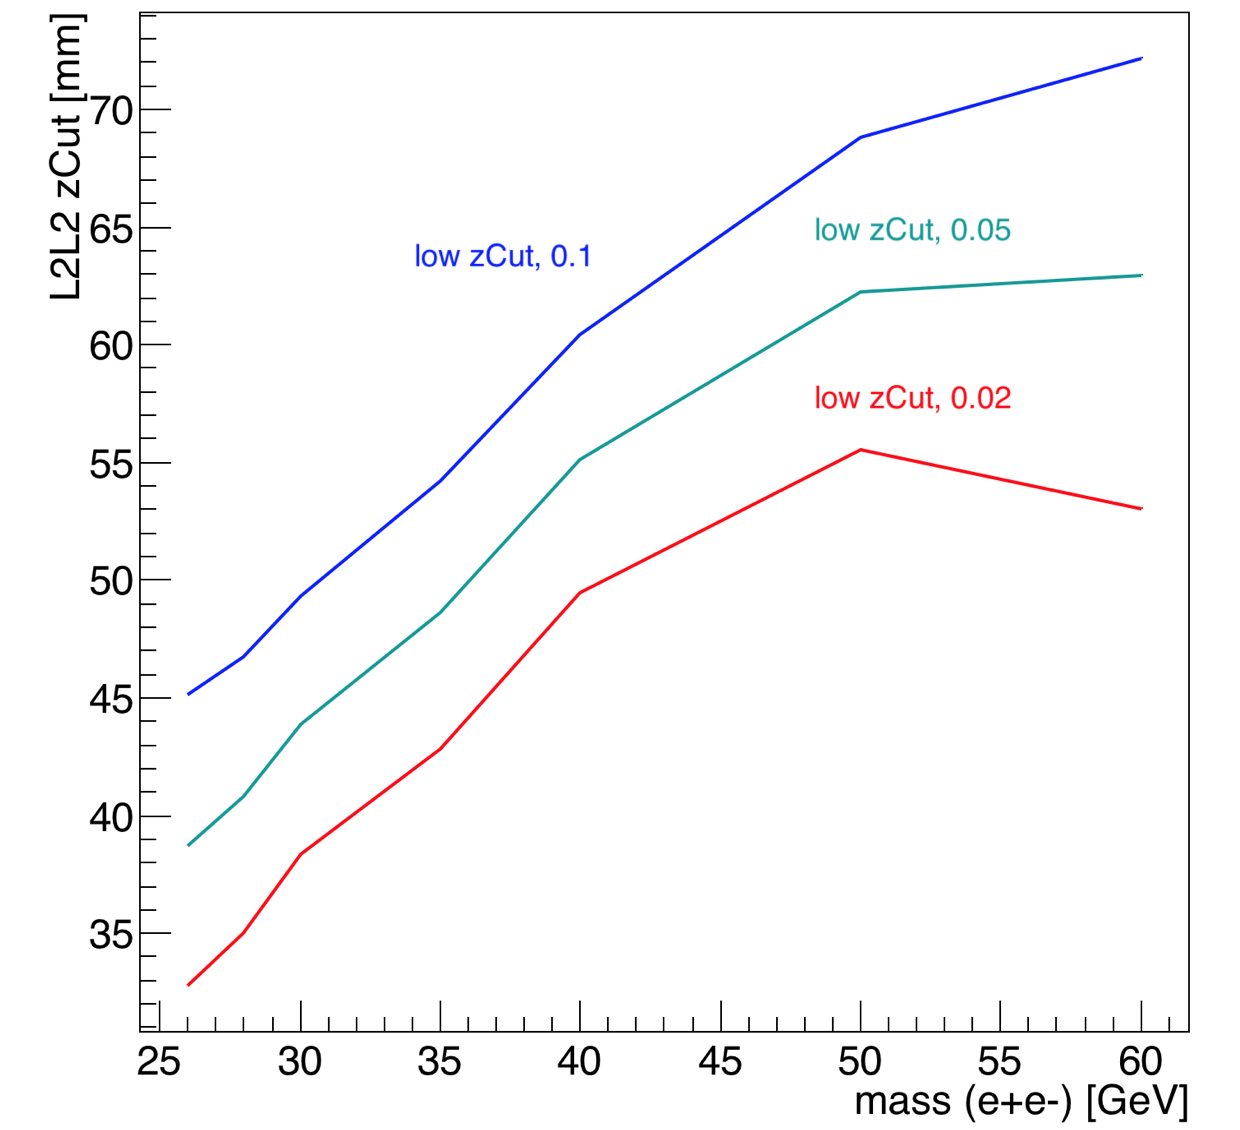
\includegraphics[width=0.8\textwidth]{plots/L2L2_proposedZcut_1p5.png}
  \caption{.}
  \label{fig:L2L2_zCut_1p5}
\end{figure} 

After all cuts are applied, the resultant z vertex distribution as a function of mass is shown in Figure~\ref{fig:zVm_L2L2_1p5}.

\begin{figure}[H]
  \centering
     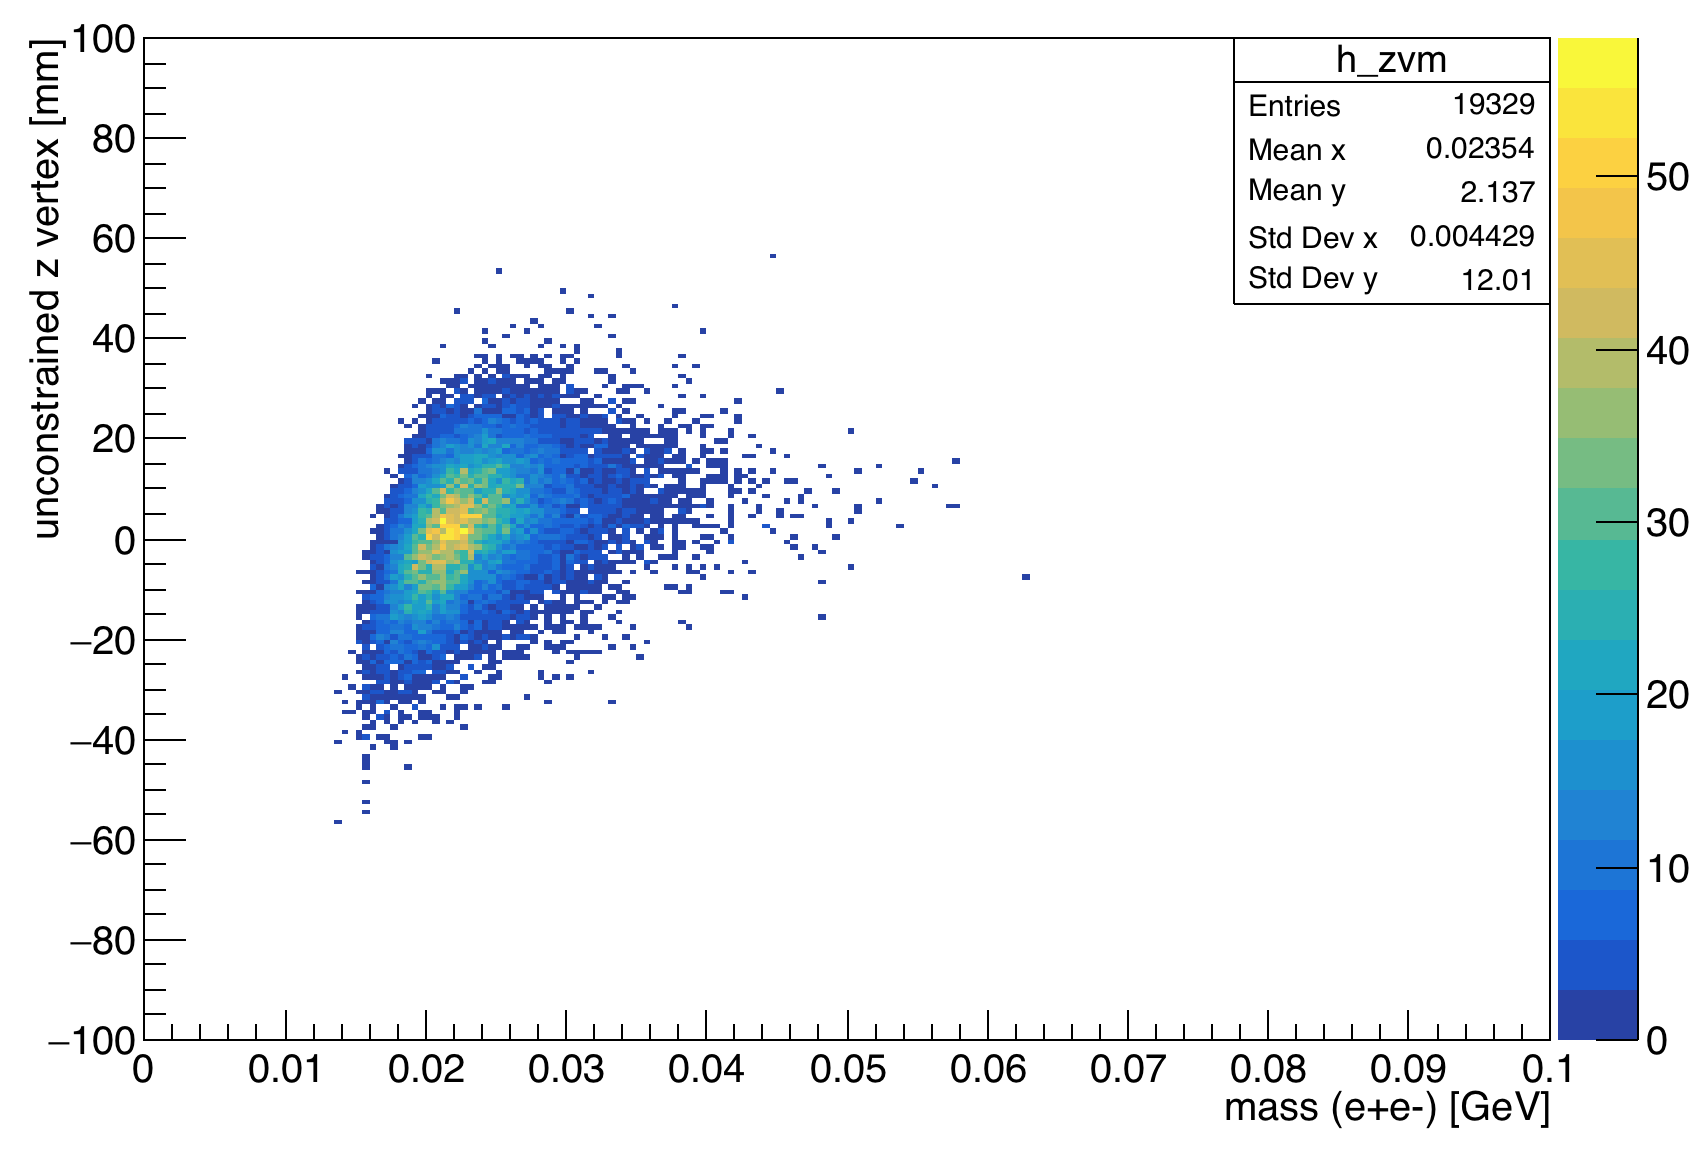
\includegraphics[width=0.8\textwidth]{plots/zVm_L2L2_1p5.png}
  \caption{Reconstructed z vertex as a function of mass for the L1L1 dataset with the first layer of the SVT at 1.5~mm from the beam. The solid red line indicates the zCut found for 10$\%$ of the data (unblinded), and the dashed red line indicates the limit at which events have a quantile greater than 0.5 with respect to the predicted background model. The purple line shows where the projected zCut will be for the full dataset after unblinding.}
  \label{fig:zVm_L2L2_1p5}
\end{figure} 

Assuming that we can remove some of the higher z background events and obtain a reasonable zCut that may optimize the signal yield, we can estimate the upper limit contribution of the L2L2 1.5~mm dataset as shown in the following Figure~\ref{fig:reach1p5_l2l2}.

\begin{figure}[H]
  \centering
     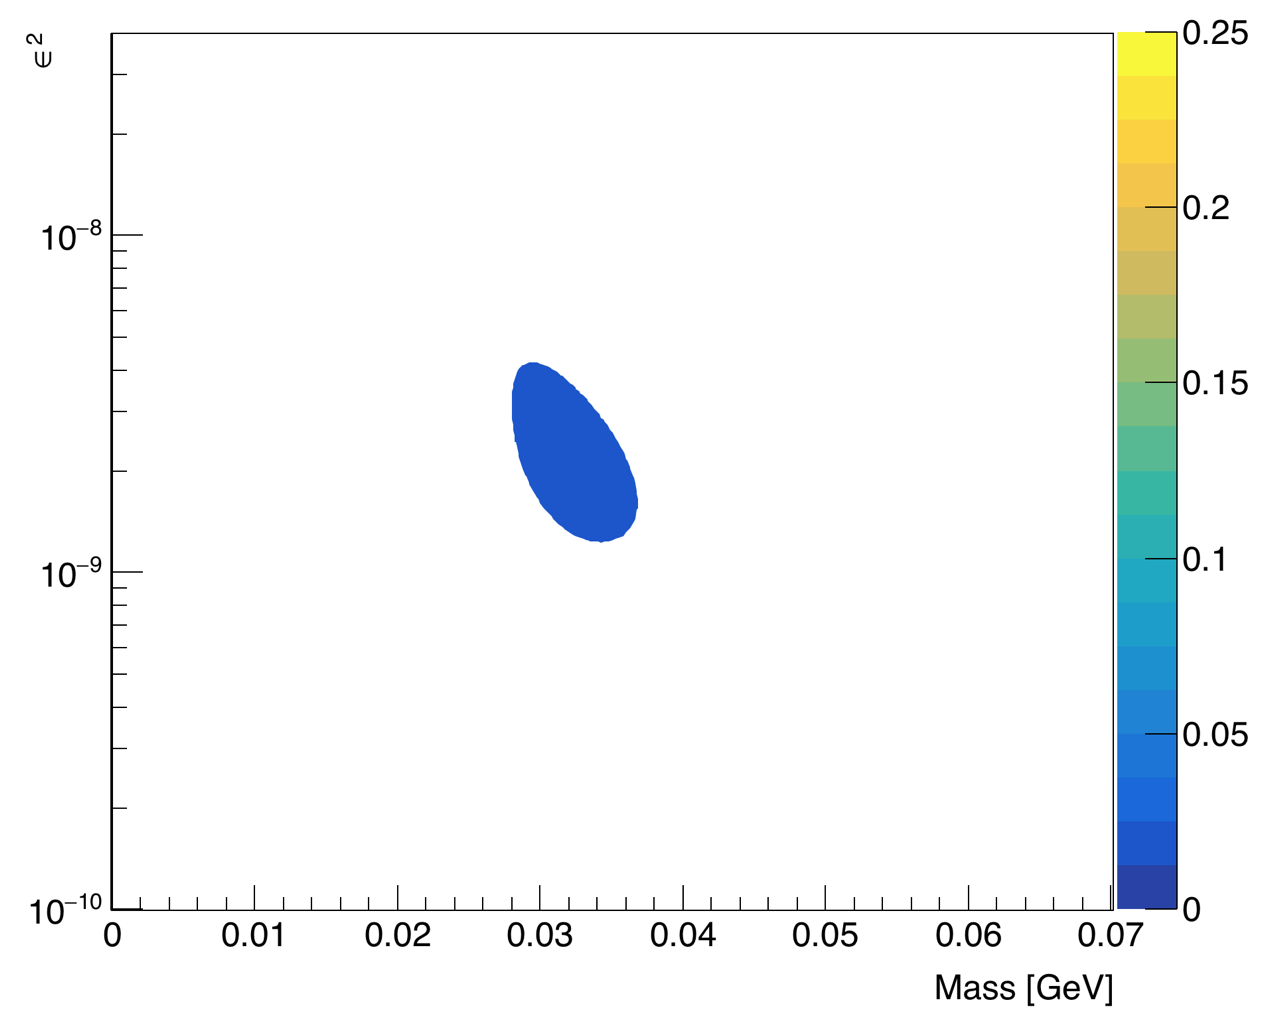
\includegraphics[width=0.8\textwidth]{plots/reachL2L2_1p5.png}
  \caption{The expected signal yield for the full 100$\%$ dataset with the L2L2 1.5~mm data.}
  \label{fig:reach1p5_l2l2}
\end{figure} 

This upper limit assumes that we can obtain the mass resolution as found in the L1L2 dataset. If we are able to fully characterize the backgrounds of this dataset, optimize the zCut, and improve the mass resolution, then we can probe smaller couplings of the HPS reach parameter space. 
